\section{Algoritmo GRASP}


\subsection{Solución}
La idea de este algoritmo es ejecutar una serie de veces nuestro algoritmo GREEDY randomizado y buscar en cada solución una mejora local, guardando la mejor solución hasta el momento.
Gracias a la parte aleatoria del algoritmo Greedy, aplicar repetidas veces este algoritmo nos otorga soluciones obtenidas de distinta forma en cada caso, de distintas partes del espectro de soluciones, las cuales llevamos a mínimos locales para allí comparar sus cardinales y quedarnos con la menor. Nuestra esperanza es, entonces, poder caer en un mínimo global.
Esa randomización se debe a que el método por el cuál dicho algoritmo goloso elige siempre el mejor valor bajo su criterio, es ahora aleatorizada seleccionando al azar entre los primeros k elementos de la
lista de nodos a ser considerado dominante.\\
Hablándo un poco más en lenguaje de GRASP, la RCL (Restricted Candidate List) es la lista que contiene un conjunto de posibles mejores candidatos según el criterio de nuestro Greedy y de ella eligiremos un valor al azar. Esta lista decidimos armarla desde el algoritmo Greedy.
Para ello, agregamos en el algoritmo Greedy que reciba por parámetro dicho k, de forma tal que al momento de elegir el próximo nodo, en vez de elegir el primero de los nodos ordenados por la cantidad de adyacentes
sin dominar, ahora elige la posición i, que será el número obtenido pseudo-aleatoriamente a través de la función random entre 0 y k. En caso de que este k sea mayor a la cantidad de nodos considerados en la lista, 
k se definirá como la longitud de dicha lista.\\
En las heurísticas GRASP es necesario elegir un criterio de parada para que el algoritmo no se ejecute infinitamente. En nuestro caso, decidimos elegir unicamente
una cantidad de iteraciones, ya que esto nos permitió jugar libremente con ese parámetro y no preocuparnos por casos en los que
la solución inicial fuera optima y nunca se realizara mejora.


\subsection{Pseudocódigo}

\begin{codebox}
\Procname{$\proc{MCDGrasp}$ (\textbf{in} $Grafo$, \textbf{in} $k$)}{ConjDominante}{Conj}
\li	mejorSolucion = TodosLosVertices
\li \textbf{Para} i=0 hasta k \Do
\li 	instanciaSolucionGreedyRandomized = MCDGreedy(grafo,k)
\li	nuevaSolucion = MCDLocalSearch(instanciaSolucionGreedyRandomized)
\li 	\textbf{Si} cantNodosDominantes(nuevaSolucion) $<$ cantNodosDominantes(mejorSolucion)  \Do
\li		mejorSolucion = nuevaSolucion
\li		\textbf{Si} mejorSolucion.size() == 1 \Do
\li			\textbf{return} mejorSolucion
		\End
	\End
    \End	
\li	\textbf{return} mejorSolucion	
\end{codebox}
Comenzamos con todos los vertices como mejor solución, de forma tal que la próxima solución siempre sera mejor o igual.\\
Se debe aclarar que tanto LocalSearch como Greedy devuelven ConjuntosDominantes verdaderos, por lo que lo único que importa es la cantidad de nodos devuelta.\\

A continuación se agrega el cambio hecho en el algoritmo greedy para aleatorizar la selección de nodos:\\
\begin{codebox}
\Procname{$\proc{elegirVertice}$ (\textbf{in} $ListaVerticesORdenada$, \textbf{in} $k$)}{proxVertice}{Vertice}	
\li     \textbf{Si} k $>$ $|$ListaVerticesORdenada$|$ \Do
\li 		k = $|$ListaVerticesORdenada$|$;
\End
\li 	posiciónAElegir = random(0,k);
\li	proxVertice = ListaVerticesORdenada[posiciónAElegir]
\li 	\textbf{return} proxVertice
\end{codebox}

\subsection{Análisis de Complejidad}
Por la demostración de la complejidad de la búsqueda local, sabemos que la complejidad es: O($n^4$);\\
Por la demostración de la complejidad del goloso, sabemos que la complejidad es: O($n^3$);\\
Dentro del GRASP se realizan k iteraciones de las siguientes operaciones:
\begin{itemize}
\item Ejecutar algoritmo goloso con random
\item Ejecutar algoritmo localSearch a partir de la solución del goloso
\item Comparar mejorSolución con nuevaSolución (esta operación es en O(1) ya que tanto conseguir el tamaño de un ArrayList en Java como la comparación de enteros es en O(1)) 
\end{itemize}
Esto es O(k*(goloso + localSearch)), que resulta polinomial.\\
Entonces la complejidad resulta O(k*$n^4$);


\subsection{Tests y análisis}
Tal como hicimos con los anteriores algoritmos, acá también se tomaron los peores y los mejores casos. Como la randomización evita encontrar un peor/mejor caso per-se, se 
decidió correr los mencionados
en los puntos anteriores. Retomando un comentario anterior, GRASP te da la oportunidad de recorrer más el espacio de soluciones y buscar en cada uno una mejor versión vecinal, 
gracias a esto podemos socorrer los 
casos en donde Greedy o Greedy+LocalSearch no son óptimos gracias a esta cuota de randomización. Muchas veces esto pasa porque Greedy encuentra una solución que localmente es 
buena, lo que reduce el marco 
de posibles soluciones locales. Cuando ejecutamos GRASP, el greedy ejecutado en él notamos que devuelve un peor caso que el goloso original, pero eso provee un espacio vecinal 
mucho más grande para que el Local
Search pueda trabajar. \\
Al igual que en la búsqueda local, en este algoritmo tambien se incrementa la cantidad de operaciones a medida
que se incrementa la cantidad de conjuntos dominantes devuelto por la solución greedy.\\
Cabe recordar que en cada iteración, el algoritmo greedy retorna una solución de las k*$|$conjuntoDominante$|$ posibles soluciones, que después se buscará localmente una mejora 
en caso de existir a través del camino elegido.\\
Antes de hacer los gráficos, deberíamos calcular cual es el peor caso para este algoritmo. Sin embargo, el mismo depende de dos cosas:
La solución random generada por el algoritmo goloso cuando se usa el valor de k. Esto es importante, ya que mientras esa solución sea generada de forma pseudo-random, menor cantidad
de operaciones va a haber en la búsqueda local.
A continuación se muestran algunos de los ejemplos realizados para distintas cantidades de nodos, distintas iteraciones obteniendo resultados en los peores y mejores casos.


\begin{center}
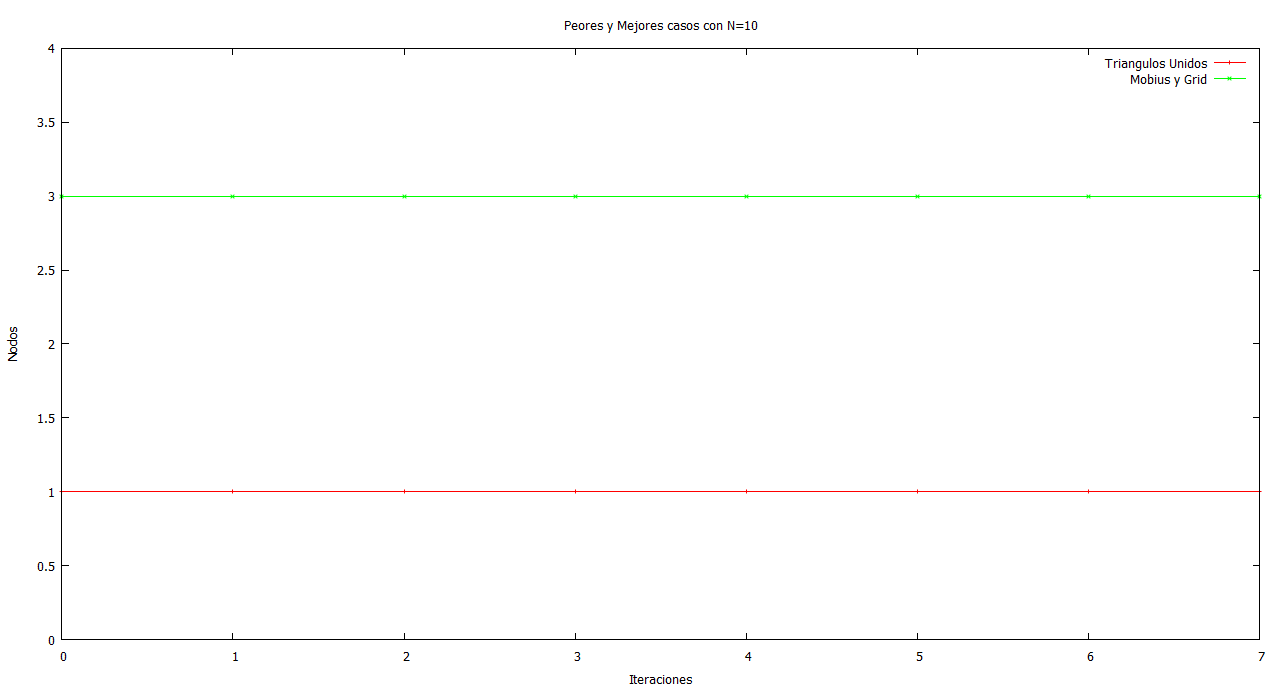
\includegraphics[width=17cm]{./graficos/grasp/peoresymejoresn10.png}\\
Peores y mejores casos con n = 10.
\end{center}

\begin{center}
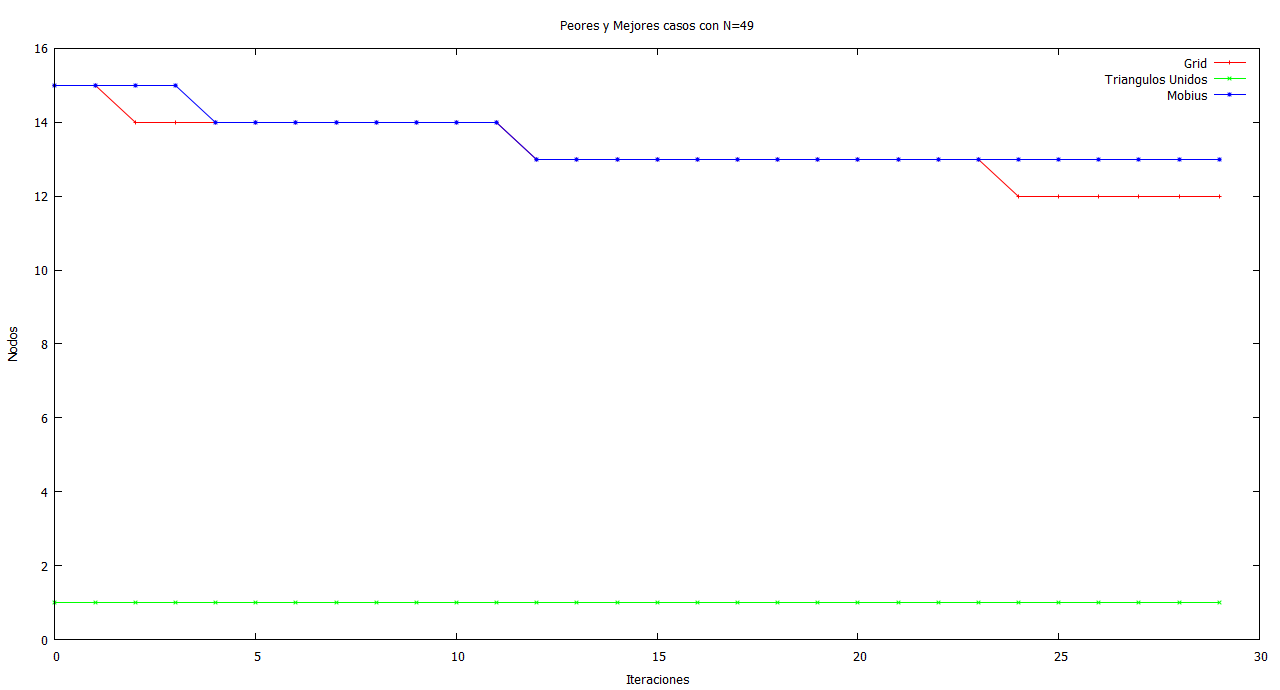
\includegraphics[width=17cm]{./graficos/grasp/peoresymejoresn49.png}\\
Peores y mejores casos con n = 49.
\end{center}

\begin{center}
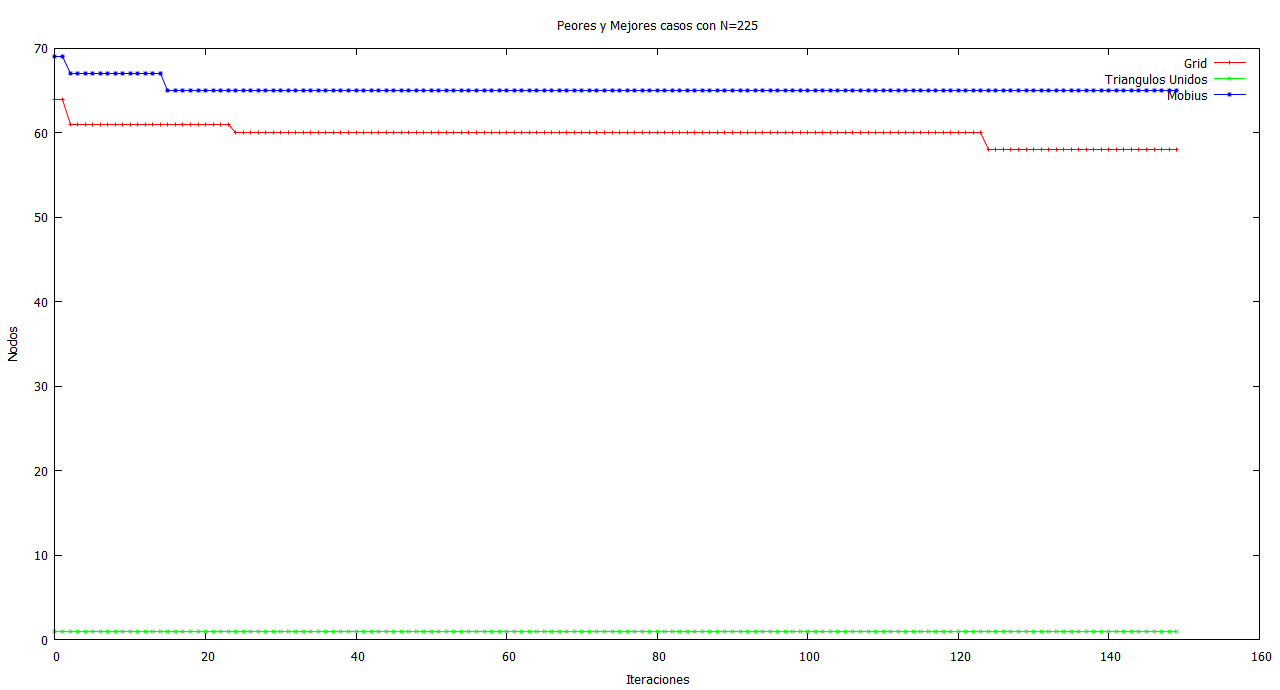
\includegraphics[width=17cm]{./graficos/grasp/peoresymejoresn225.png}\\
Peores y mejores casos con n = 225.
\end{center}

%\begin{center}
%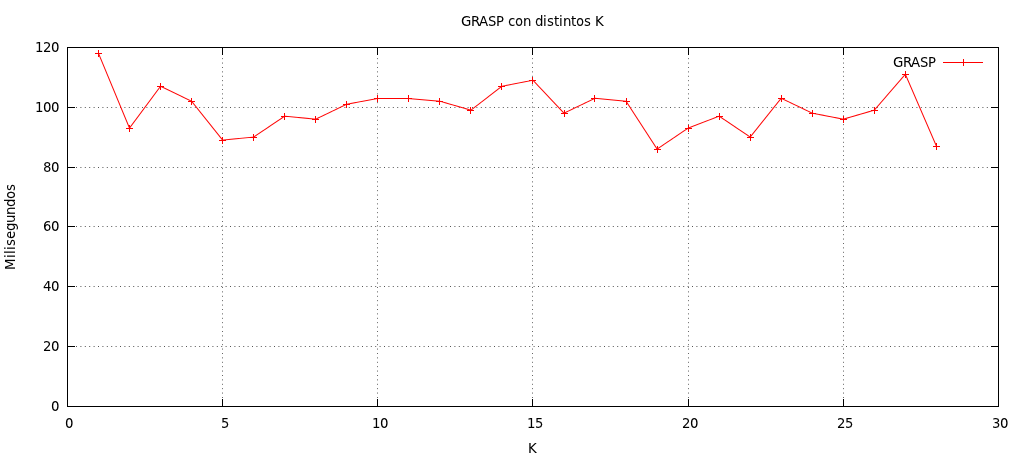
\includegraphics[width=15cm]{./graficos/GRASP_distintosK.png}\\
%Peores y mejores casos con n = 500.
%\end{center}

Como se puede ver en los gráficos, la cantidad de nodos no se reduce por utilizar un k más grande. Esto es importante pero veamos por qué.
En la i-esima iteración, GRASP le pide a Greedy que obtenga una nueva solución tomando siempre, en cada iteración de este último, de los primeros k posibles un nodo random como 
próximo elemento a ser considerado como dominante, y una vez que el conjunto sea dominante, será mejorado con local search.\\
Ahora entonces tenemos una nueva solución, independiente de la i-1-esima iteración. Notemos que esta solución no es necesariamente mejor a la anterior, 
esto se debe a que el elemento obtenido de la RCL puede ser bastante malo según el criterio greedy y por lo
tanto se obtiene un conjunto grande, que la búsqueda local no alcanza a mejorar del todo. Por otro lado, si el tamaño de la
RCL es muy chico, la solución inicial greedy randomizada va a ser muy similar a la greedy clásico (no randomizado). Esto nos
llevaría a explorar una cantidad más acotada de vecindarios de soluciones al momento de aplicar la búsqueda local.
Entonces concluimos que al momento de elegir el k, notar que con pocos k ya se puede obtener lo que sería el ideal, pero sin embargo es conveniente utilizar una RCL
más grande para abrir el panorama de soluciones.

A continuación se agrega un gráfico para evaluar los tiempos para distintos k con distintos nodos del conjunto de familias detallado en los gráficos anteriores:


\begin{center}
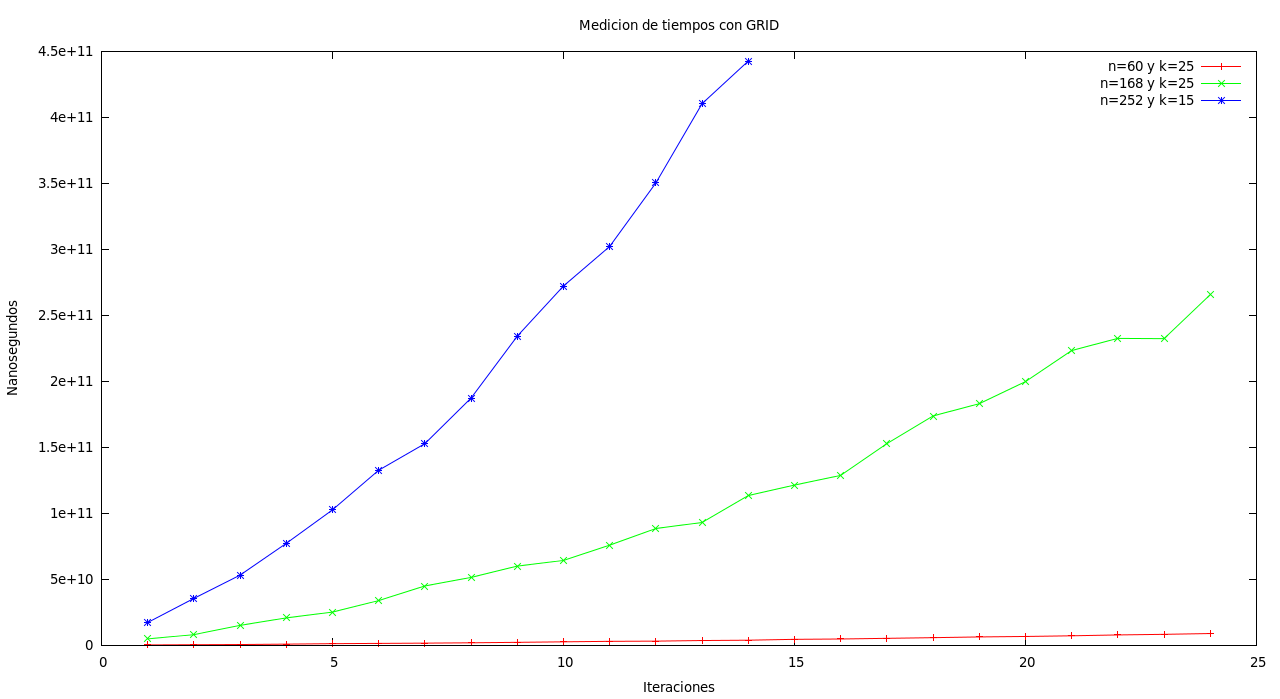
\includegraphics[width=17cm]{./graficos/grasp/medicionesdetiempocongrid.png}\\
Flia de grafo Grid perteneciente al peor caso con n=60, n=168, n=252 con k $<$ 25
\end{center}

%\begin{center}
%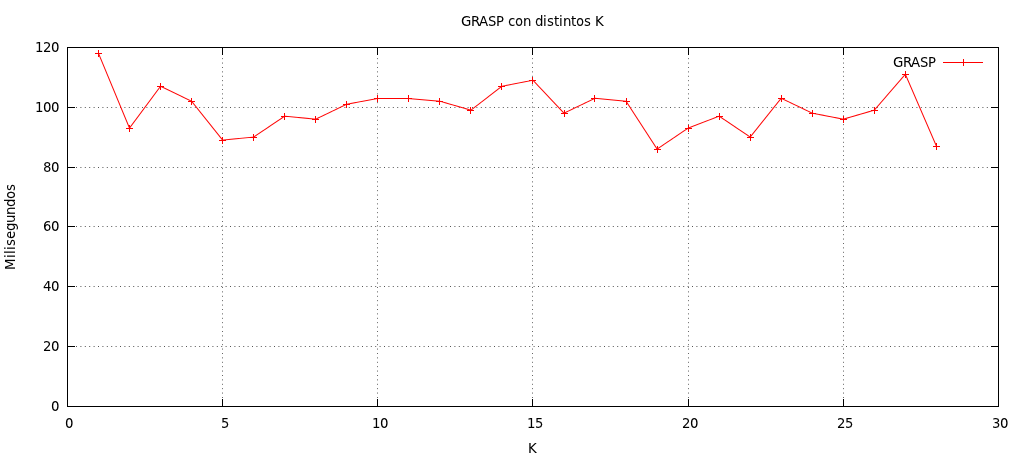
\includegraphics[width=17cm]{./graficos/GRASP_distintosK.png}\\
%Flia de grafo Triangulos Unidos perteneciente al mejor caso con n=12, n=60, n=168, n=252 con $<$ 25
%\end{center}

%VER QUE ES MUY RAPIDO ESTE, O SEA NO ES SOLO ES MEJOR EN CANT DE NODODS SI NO EN TIEMPO

Como era esperable, la relación es lineal. Esto es ya que el K multiplica como constante y esta es siempre menor a n, ya que correr con un k mayor a n no tendría sentido práctico. Las pequeñas diferencias se deben a que al depender de otros algoritmos como ser: Greedy y LocalSearch, que tienen una condición de corte distinta a la de este algoritmo, puede pasar que terminen antes o tarden más. Por ejemplo, en caso de que greedy con un k, elija en tres iteraciones un conjunto dominante minimal y sin embargo para otro k elija en más iteraciones.\\
Tomamos k chicos, ya que como vimos con k muy grandes no significa mejores, resultados, y de esta forma mostramos un gráfico útil al momento de elegir qué algoritmo correr.\\

A continuación se agrega un gráfico con los tiempos de corrida para distintos n de la familia Greed comparado con la cota superior:

\begin{center}
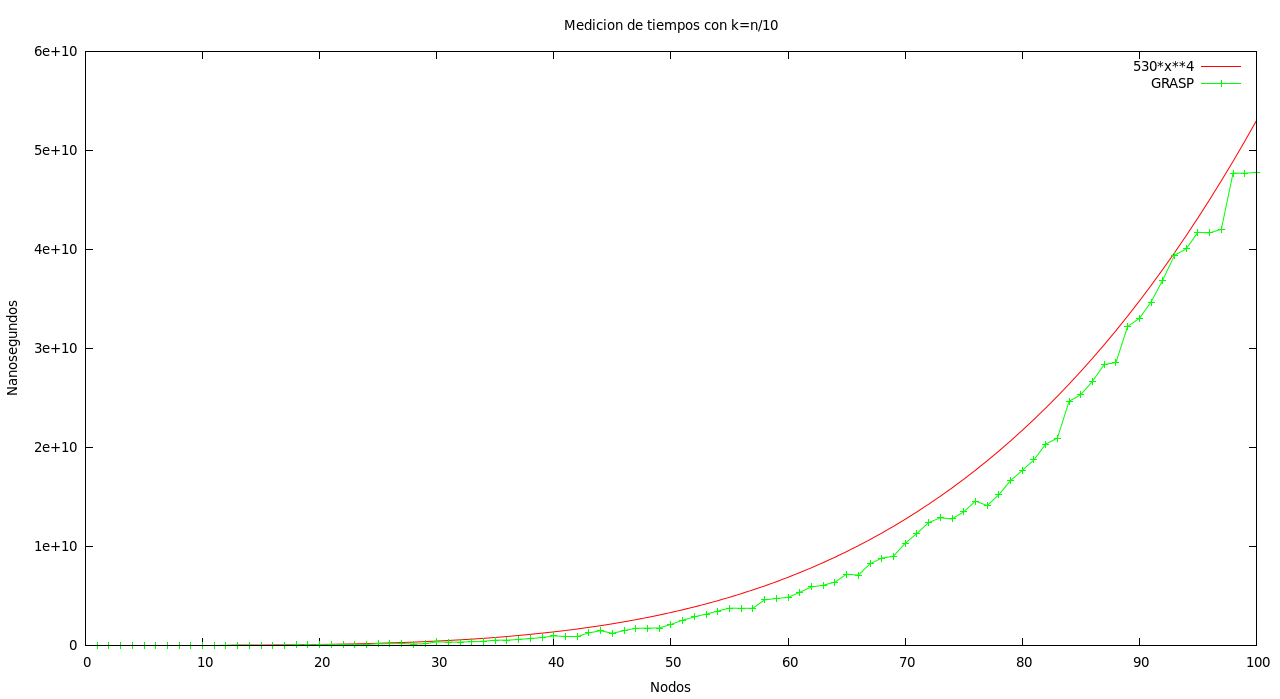
\includegraphics[width=17cm]{./graficos/grasp/tiempocondistintosngreedconx4.png}\\
Flia de grafo Triangulos Unidos perteneciente al mejor caso con n=12, n=60, n=168, n=252 con $<$ 25
\end{center}

Como se puede ver, mantenemos la cota mencionada. Las pequeñas diferencias que hacen que no sea completamente paralela, se deben a lo mencionado en el párrafo anterior, ya que estámos trabajando con un grafo random. Sin embargo, es interesante ver que aunque pertenezca a O($n^4$), no es despreciable ni el k ni el hecho de que dentro del ciclo realice una ejecución de GREEDY $\in$ O($n^3$)



%-------------------------------------------------------------------------- VERSION ANTERIOR QUE NO IRIA -----------------------------------------------------------------------------




%Ahora se presenta un algoritmo con un mismo grafo corrido n veces con k random cada vez

%\begin{center}
%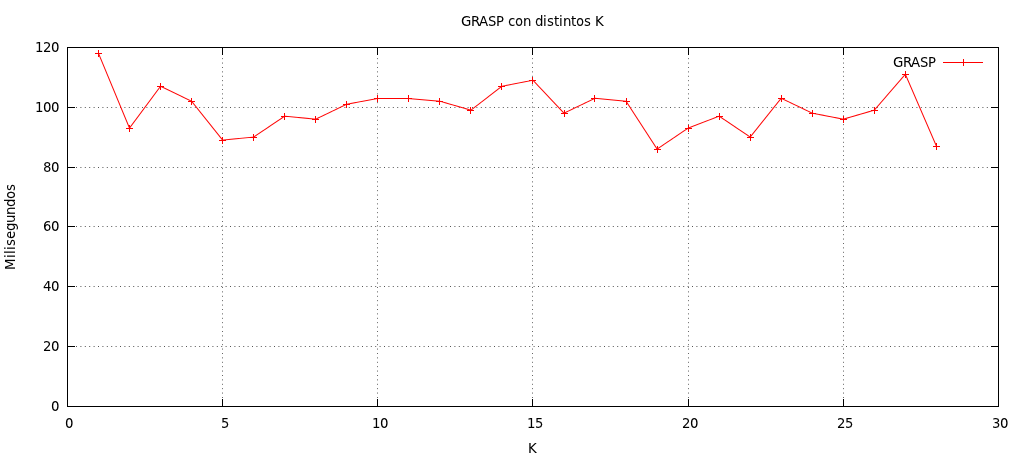
\includegraphics[width=15cm]{./graficos/GRASP_distintosK.png}
%\end{center}

%Como se puede notar en la imágen, el tiempo no varía ya que k se comporta como una constante al ser siempre menos a la cantidad de nodos, por lo que en caso de saber valores %de la entrada en los que sabemos
%que Greedy se comportaría mal al elegir siempre el mejor a partir de su estrategia, elegir un k más grande para poder elegir entre más nodos aleatoriamente, no arruina el tiempo de procesamiento.

%Ahora se presenta un algoritmo con distintos grafos corrido cada uno con k = 5,10,15,20

%\begin{center}
%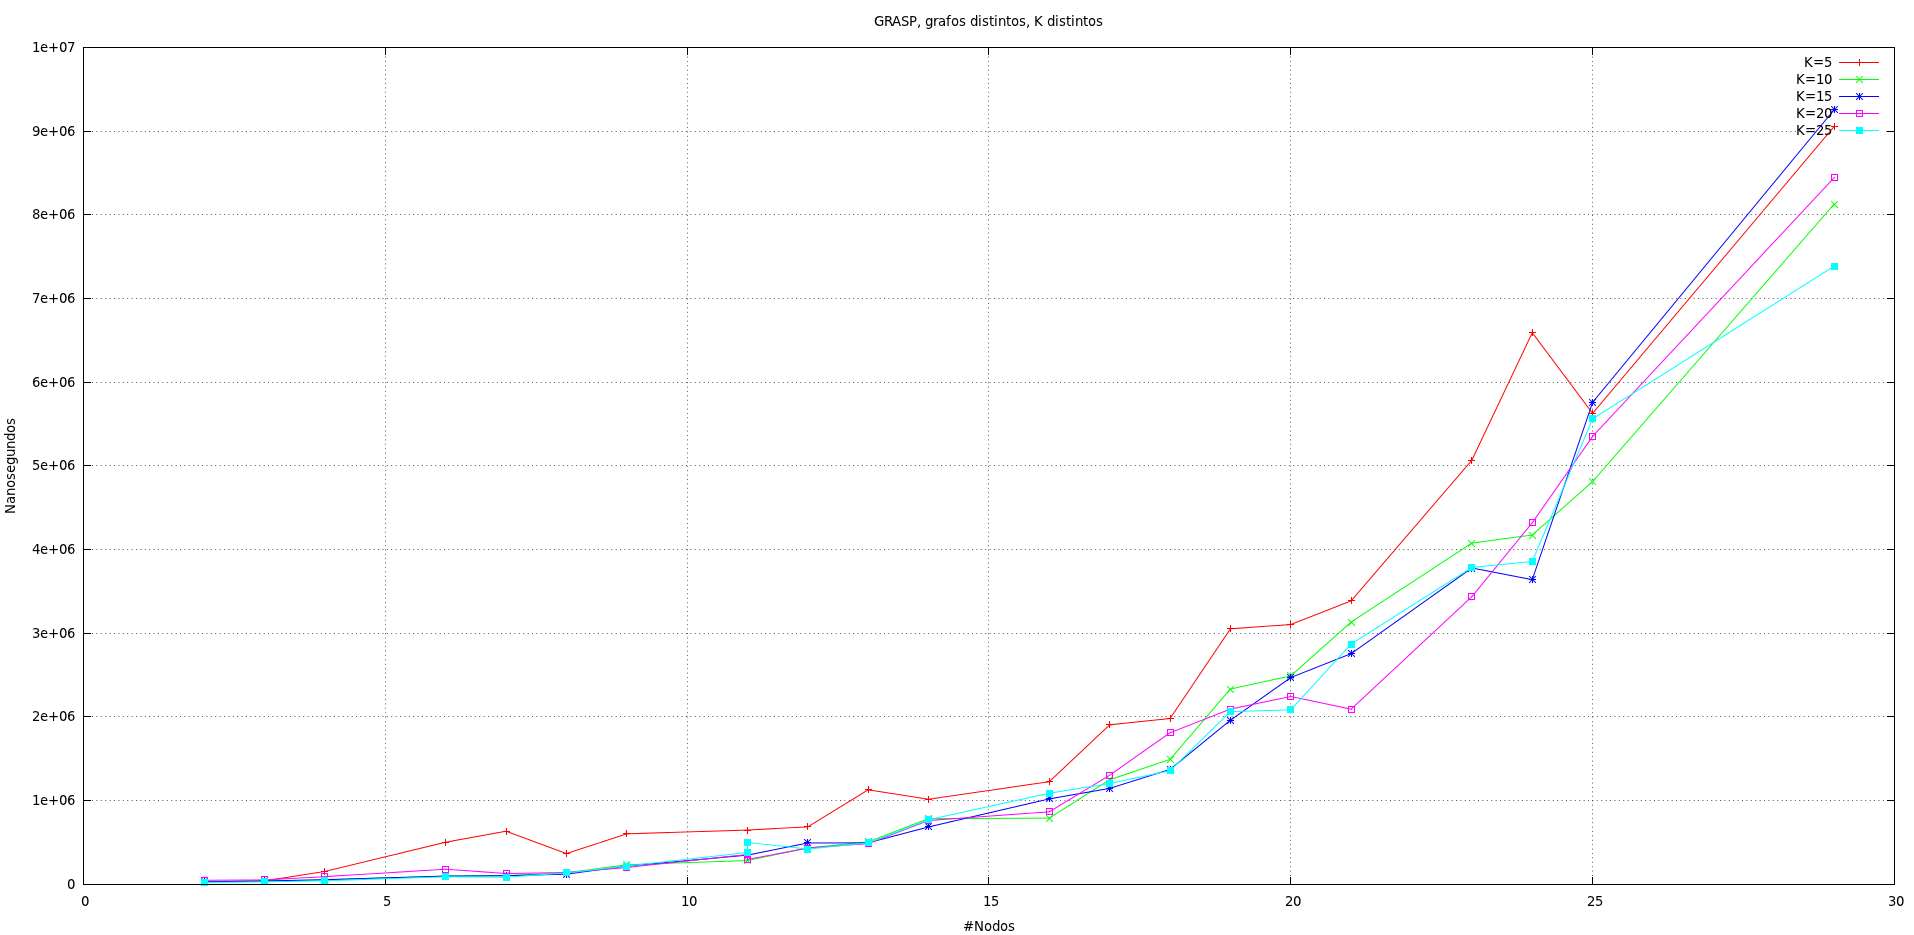
\includegraphics[width=15cm]{./graficos/GRASP_distGrafos_distK.png}
%\end{center}

%Tal como era esperado el algorimto hace menos operaciones cuando tiene menos nodos y el k multiplica el tiempo como una constante.
%Sin embargo, es necesario tener en cuenta que, al depender de otros algoritmos como ser: Greedy y LocalSearch, que tienen una condición de corte distinta a la de este algoritmo, puede pasar que terminen antes o tarden más.
%Es así que se explican la falta de paralelismo exacto de los gráficos. Por ejemplo, en caso de que greedy con un k, elija en tres iteraciones un conjunto dominante minimal y sin embargo para otro k elija en más iteraciones.
